% Chapter 7 (Prognostic Performance): schematic follow-up timelines. Not data.
{\hpdiagramsizes
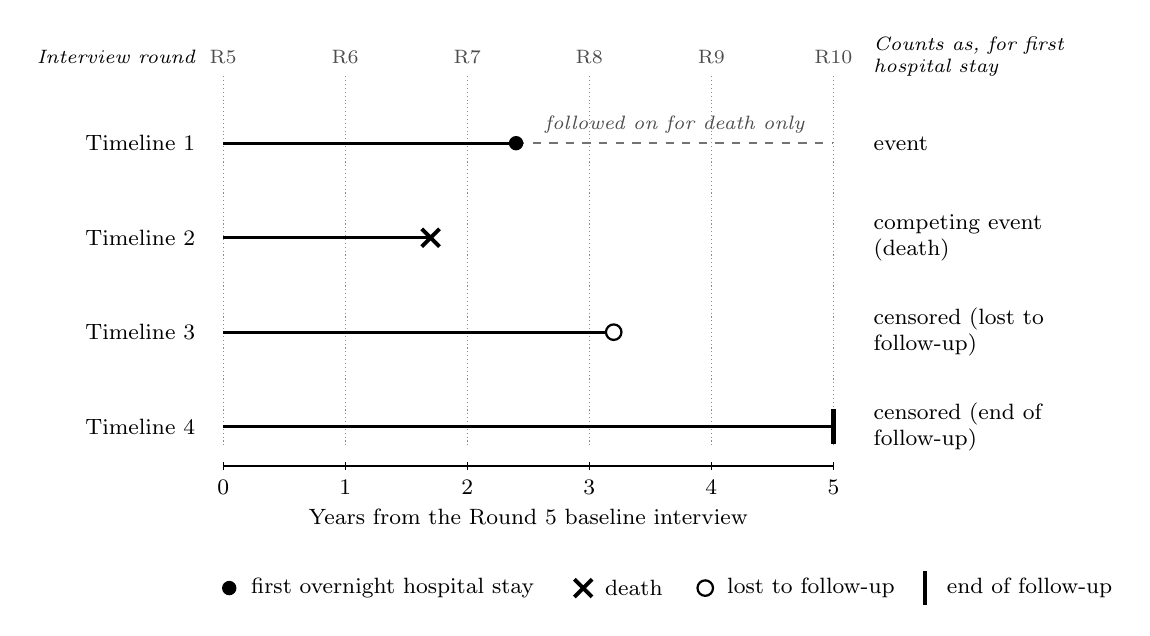
\begin{tikzpicture}[x=1.55cm, y=1cm, font=\footnotesize]
  % interview rounds: one a year from the Round 5 baseline
  \foreach \t/\r in {0/R5, 1/R6, 2/R7, 3/R8, 4/R9, 5/R10} {
    \draw[densely dotted, black!45] (\t, 0.35) -- (\t, -4.35);
    \node[font=\scriptsize, black!70] at (\t, 0.6) {\r};
    \draw (\t, -4.55) -- (\t, -4.65) node[below] {\t};
  }
  \node[font=\scriptsize\itshape, anchor=east] at (-0.15, 0.6) {Interview round};
  \draw (0, -4.6) -- (5, -4.6);
  \node at (2.5, -5.25) {Years from the Round~5 baseline interview};
  % right-hand column header
  \node[font=\scriptsize\itshape, anchor=west, text width=2.8cm] at (5.25, 0.6) {Counts as, for first hospital stay};

  % timeline 1: first overnight hospital stay, then still followed for death
  \node[anchor=east] at (-0.15, -0.5) {Timeline 1};
  \draw[very thick] (0, -0.5) -- (2.4, -0.5);
  \draw[thick, dashed, black!55] (2.4, -0.5) -- (5, -0.5);
  \fill (2.4, -0.5) circle (2.6pt);
  \node[font=\scriptsize\itshape, black!70, above] at (3.7, -0.5) {followed on for death only};
  \node[anchor=west, text width=2.8cm] at (5.25, -0.5) {event};

  % timeline 2: dies before any stay (competing event)
  \node[anchor=east] at (-0.15, -1.7) {Timeline 2};
  \draw[very thick] (0, -1.7) -- (1.7, -1.7);
  \draw[line width=1.4pt] (1.7, -1.7) ++(-3.2pt, -3.2pt) -- ++(6.4pt, 6.4pt)
                          (1.7, -1.7) ++(-3.2pt,  3.2pt) -- ++(6.4pt, -6.4pt);
  \node[anchor=west, text width=2.8cm] at (5.25, -1.7) {competing event (death)};

  % timeline 3: lost to follow-up
  \node[anchor=east] at (-0.15, -2.9) {Timeline 3};
  \draw[very thick] (0, -2.9) -- (3.2, -2.9);
  \draw[thick, fill=white] (3.2, -2.9) circle (2.8pt);
  \node[anchor=west, text width=2.8cm] at (5.25, -2.9) {censored (lost to follow-up)};

  % timeline 4: reaches end of follow-up event-free
  \node[anchor=east] at (-0.15, -4.1) {Timeline 4};
  \draw[very thick] (0, -4.1) -- (5, -4.1);
  \draw[line width=1.6pt] (5, -3.88) -- (5, -4.32);
  \node[anchor=west, text width=2.8cm] at (5.25, -4.1) {censored (end of follow-up)};

  % legend: shapes, not colour
  \begin{scope}[shift={(0, -6.15)}]
    \fill (0.05, 0) circle (2.6pt);
    \node[anchor=west] at (0.15, 0) {first overnight hospital stay};
    \draw[line width=1.4pt] (2.95, 0) ++(-3.2pt, -3.2pt) -- ++(6.4pt, 6.4pt)
                            (2.95, 0) ++(-3.2pt,  3.2pt) -- ++(6.4pt, -6.4pt);
    \node[anchor=west] at (3.05, 0) {death};
    \draw[thick, fill=white] (3.95, 0) circle (2.8pt);
    \node[anchor=west] at (4.05, 0) {lost to follow-up};
    \draw[line width=1.6pt] (5.75, 0.22) -- (5.75, -0.22);
    \node[anchor=west] at (5.85, 0) {end of follow-up};
  \end{scope}
\end{tikzpicture}}
